
\newfloatcommand{capbtabbox}{table}[][\FBwidth]

We evaluate our custom compression scheme against Morden, Ropsten and Frontier blockchains.
Table \ref{tab:origvscustom} shows the compression gains obtained after using our technique.
As can be seen, savings as much as 40\% can be seen on the main blockchain demonstrating the usefulness
of our technique.
\begin{figure*}[!t]
\CenterFloatBoxes
\begin{floatrow}
\capbtabbox{
	\begin{tabular}{ >{\bfseries}c| p{1.5cm} | p{1.5cm} | p{1.5cm} |p{1.5cm}}
	Blockchain& {Size of Original File (MB)} & {\par{Size of Custom format \newline (MB)}} & {Size of Custom format with Huffman Encoding (MB)} \\
  \hline
  Ropsten & 98.6 & 47.8  & 44.4 \\
  Morden & 2160 & 1135.4 &1068.9  \\
  Frontier  & 3434.6  & 2069 & 2037.5 \\ 
\end{tabular}
%\begin{tabular}{ >{\bfseries}c| p{1.5cm} | p{1.5cm} | p{1.5cm} |p{1.5cm} |p{1.5cm} }
%	Blockchain& {Size of Original File (MB)} & {\par{Size of Custom format \newline (MB)}} & {Size of Custom format with Huffman Encoding (MB)} & \par{Percentage Gain without Huffman Encoding}  & \par{Percentage Gain with Huffman Encoding} \\
%  \hline
%  Ropsten & 98.6 & 47.8  & 44.4 &51.5  & 55.0\\
%  Morden & 2160 & 1135.4 &1068.9 & 47.4 & 50.5 \\
%  Frontier  & 3434.6  & 2069 & 2037.5 & 39.6 & 40.7\\
%\end{tabular}
}{
\caption{Compression using our custom format with and without Huffman encoding} 
\label{tab:origvscustom}
}
\ffigbox{
	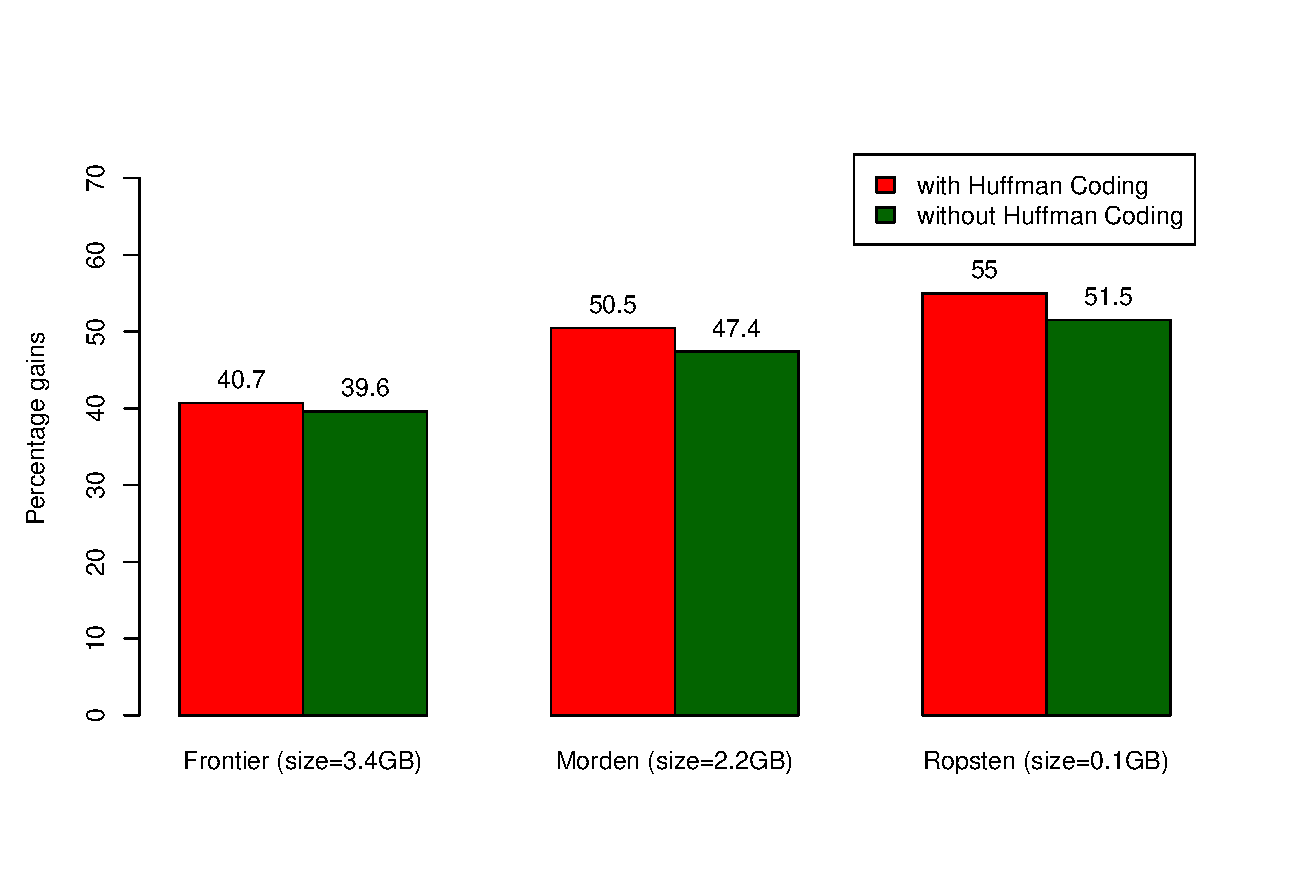
\includegraphics[scale=0.5]{plots/customgains}
	%\rule{3cm}{3cm}
}{ \caption{Percentage gains}
}
\end{floatrow}
\end{figure*}

As mentioned earlier, we do not aim to compete against the existing compressing tools that are mature.
However, we provide a comparative evaluation of our tool against gzip, bzip2 and xz. 

\paragraph{Ropsten}
Table~\ref{tab:compropsten} 
shows the additional compression savings that were possible by compressing 
our custom format using gzip, bzip2 and xz

\begin{table*}[!t]
\centering
\captionsetup{justification=centering}
\begin{tabular}{ >{\bfseries}c| p{2cm} | p{2cm} |p{2cm} | p{1.5cm} | p{1.5cm} }
	Program & {Compressed Size of Original File (MB)} & {Compressed Size on Custom format (MB)} & {Compressed Size on Custom format with Huffman Encoding (MB)}& Percentage Gain without Huffman Encoding & Percentage Gain with Huffman Encoding\\
  \hline
  gzip  & 33.4 & 27.5 & 29.4 & 17.7 & 12.0 \\
  bzip2 & 31.0 & 26.7 & 28.6 & 13.9 & 7.8  \\
  xz   & 27.8 & 22.4 &  23.3 & 19.4 & 16.2 \\
\end{tabular}
\caption{Compression of Ropsten testnet. \\ Original Size = 98.6MB. Custom format size = 47.8MB}
\label{tab:compropsten}
\end{table*}

\paragraph{Morden}
Table~\ref{tab:compmorden} 
shows the additional compression savings that were possible by compressing 
our custom format using gzip, bzip2 and xz

\begin{table*}[!t]
\centering
\captionsetup{justification=centering}
\begin{tabular}{ >{\bfseries}c| p{2cm} | p{2cm} | p{2cm} | p{1.5cm} | p{1.5cm} }
	Program & {Compressed Size of Original File (MB)} & {Compressed Size on Custom format (MB)} & {Compressed Size on Custom format with Huffman Encoding (MB)} & Percentage Gain without Huffman Encoding & Percentage Gain with Huffman Encoding \\
  \hline
  gzip  & 812.2 & 701.3 & 739.6 & 13.7 & 9.0 \\
  bzip2 & 762.9 & 685.6 & 725.8 & 10.1 & 5.0 \\
  xz   & 686.7 & 599.2 &  620.7 & 12.7 & 9.6 \\
\end{tabular}
\caption{Compression of Morden testnet. \\Original Size = 2160MB. Custom format size = 1135.4MB}
\label{tab:compmorden}
\end{table*}

\paragraph{Frontier}
Table~\ref{tab:compfrontier} 
shows the additional compression savings that were possible by compressing 
our custom format using gzip, bzip2 and xz

\begin{table*}[!t]
	\centering
\captionsetup{justification=centering}
\begin{tabular}{ >{\bfseries}c| p{2cm} | p{2cm} | p{2cm} | p{1.5cm} | p{1.5cm} }
	Program & {Compressed Size of Original File (MB)} & {Compressed Size on Custom format without Huffman Encoding (MB)} & {Compressed Size on Custom format with Huffman Encoding (MB)} &Percentage Gain without Huffman Encoding & Percentage Gain with Huffman Encoding\\
  \hline
  gzip  & 1807.1 & 1481.1 & 1627.9 & 18.0 & 10.1 \\
  bzip2 & 1751.3 & 1474.6 & 1590.0 & 15.8 & 9.2 \\
  xz   & 1541.8 & 1367.6 & 1398.7 & 11.3  & 9.3 \\
\end{tabular}
\caption{Compression of Frontier mainnet. \\ Original Size = 3434.6MB. Custom format size = 2069MB}
\label{tab:compfrontier}
\end{table*}


\begin{figure}[H]
	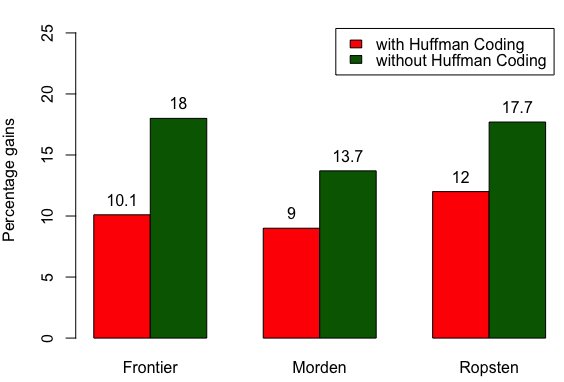
\includegraphics[scale=0.45]{plots/gzip}
	\caption{Additional compression gains (\%) using gzip}
	\label{fig:gzip}
\end{figure}
We summarize the additional compression gains in Figure~\ref{fig:gzip}, Figure~\ref{fig:bzip2} and Figure~\ref{fig:xz}. 
As we can see, the results are encouraging and show room for improvement.

\begin{figure}[H]
	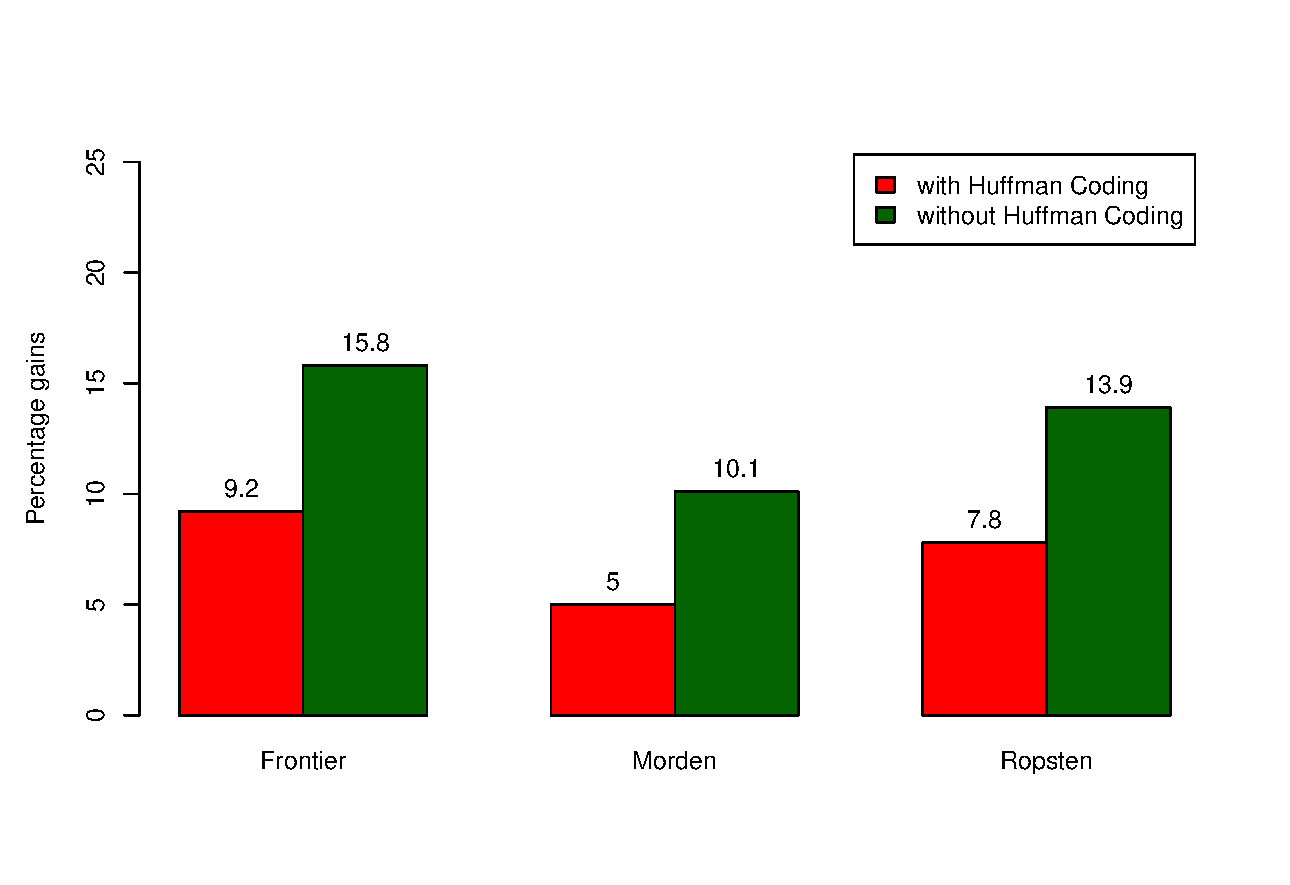
\includegraphics[scale=0.45]{plots/bzip2}
	\caption{Additional compression gains (\%) using bzip2}
	\label{fig:bzip2}
\end{figure}
\begin{figure}[H]
	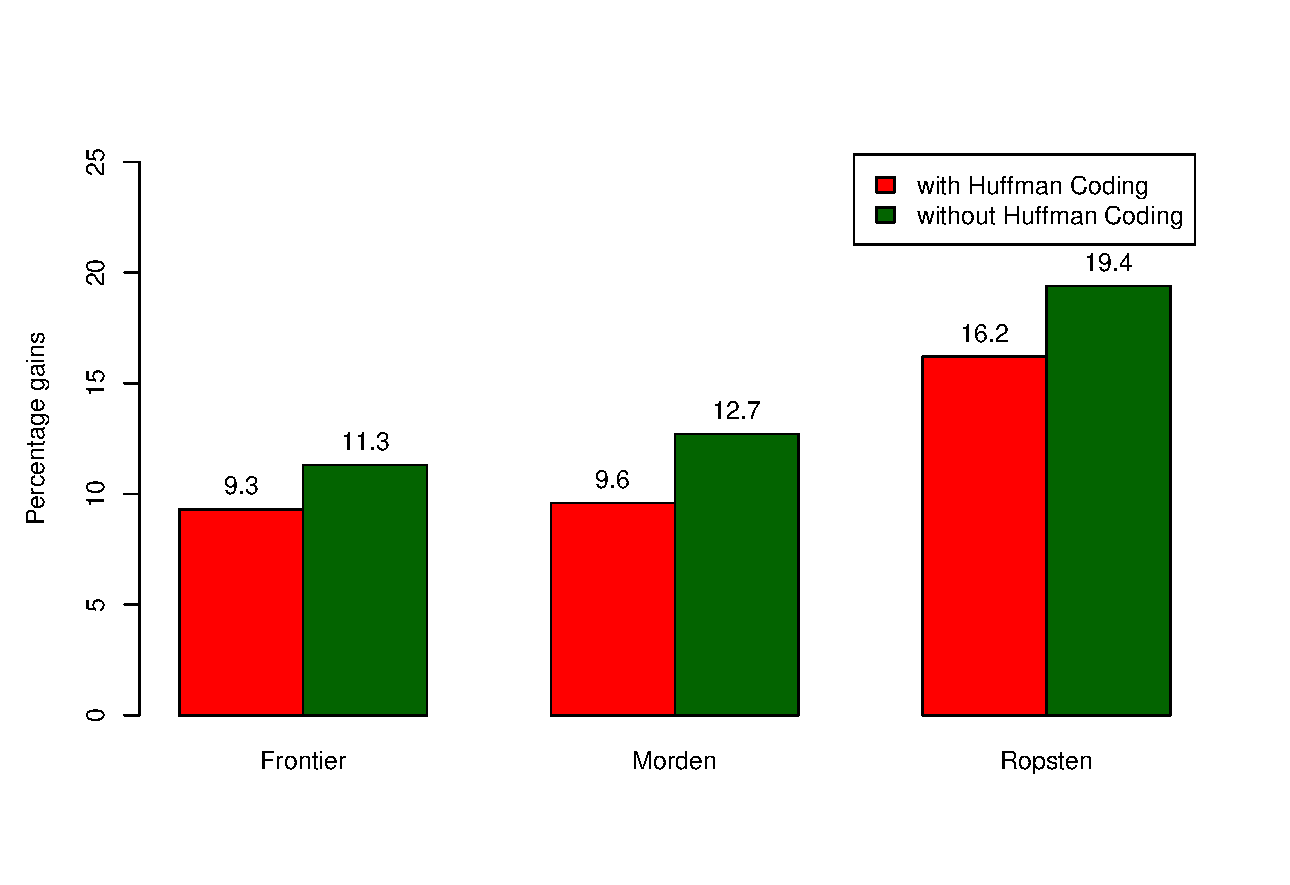
\includegraphics[scale=0.45]{plots/xz}
	\caption{Additional compression gains (\%) using xz}
	\label{fig:xz}
\end{figure}

